\documentclass[11pt]{article}
\usepackage[margin=1in]{geometry}
\usepackage{amsmath}
\usepackage{booktabs}
\usepackage{graphicx}
\usepackage{float}
\usepackage[hidelinks]{hyperref}
\emergencystretch=3em
\graphicspath{{figs/}}

\newcommand{\code}[1]{\texttt{#1}}

\title{Checking the flow-angle transform of the tunnel rig}
\author{Ilan Upfal}
\date{12 November 2026}

\begin{document}
\maketitle

\section*{Summary}

\code{scripts/aquire\_data/utils/coordinate\_transforms.py} turns a test
condition (motor angle, sweep angle, mounting angle) into the inclination and
angle of attack the blade sees. Every angle in
\code{data/Production\_summaries}, and every plot against those angles, comes
from it. The version of 1 October 2026 (commit \code{2965360}) was wrong.
This report describes the fix and the checks that show the fixed version is
right.

\begin{enumerate}
  \item \textbf{The 1 October version had two errors.} It rotated the wind
        vector by the sweep angle instead of rotating the blade's frame,
        which flipped the sign of every inclination. It also treated the
        mounting angle (84.105$^\circ$) as the angle of attack at motor
        0$^\circ$, which puts the chord nearly along the arm, and so it shifted
        every angle of attack by 78.21$^\circ$. At motor 120$^\circ$ it gave
        inclination $-25.7^\circ$ and angle of attack $-152.2^\circ$; the
        correct values are $+25.7^\circ$ and $+129.6^\circ$.
  \item \textbf{The fixed version agrees with every independent check.}
        \begin{itemize}
          \item It reproduces the three cases of the experimentalists' sketch.
          \item It matches a construction of the rig from explicit vectors
                to $10^{-13}$ degrees, over 15\,120 test conditions including
                non-horizontal flow.
          \item It matches the collaborator's original code on
                \code{master} exactly for horizontal flow, which is all the
                tunnel produces.
          \item It matches a hand calculation at motor 120$^\circ$.
        \end{itemize}
  \item \textbf{The tests would have caught the error.} The 21 new unit tests
        of the transform pass on the fixed code. On the 1 October code,
        1\,175 subtests fail.
  \item \textbf{The whole chain is consistent} (Section~\ref{sec:chain}),
        from the encoder counts to the summary tables. 13 more tests check it
        on all 1\,360 recorded angles of the 32 production runs. The angles
        the lab PC computed during acquisition, with \code{master}'s code,
        equal the fixed code's to $3\times10^{-14}$ degrees.
  \item \textbf{The summaries have been regenerated.} Only the two angle
        columns changed: every inclination changed sign exactly, and every
        angle of attack moved by exactly 78.21$^\circ$.
  \item \textbf{The mounting angle is confirmed.} The 84.105$^\circ$ is
        $90^\circ - 5.895^\circ$, entered on 29 September to give an angle of
        attack of $+5.895^\circ$ at motor 0. The chord is 5.9$^\circ$ off
        perpendicular to the arm, as the fixed code reads it. \code{main.py}
        now sets the 5.895$^\circ$ by name (\code{CHORD\_OFFSET\_DEG}) and
        derives the mounting angle from it; the stored value is
        bit-identical.
\end{enumerate}

%======================================================================
\section{The rig and the conventions}
%======================================================================

A motor turns a vertical shaft. A horizontal arm sticks out from the shaft,
and the blade hangs from the arm tip, root at the arm and tip below. In the
production runs the blade leans 30$^\circ$ in the vertical plane of the arm,
with its tip back toward the shaft, and its chord is nearly perpendicular
to the arm. All 32 production runs record sweep $-30^\circ$ and mounting
angle 84.105$^\circ$.

\begin{figure}[H]
  \centering
  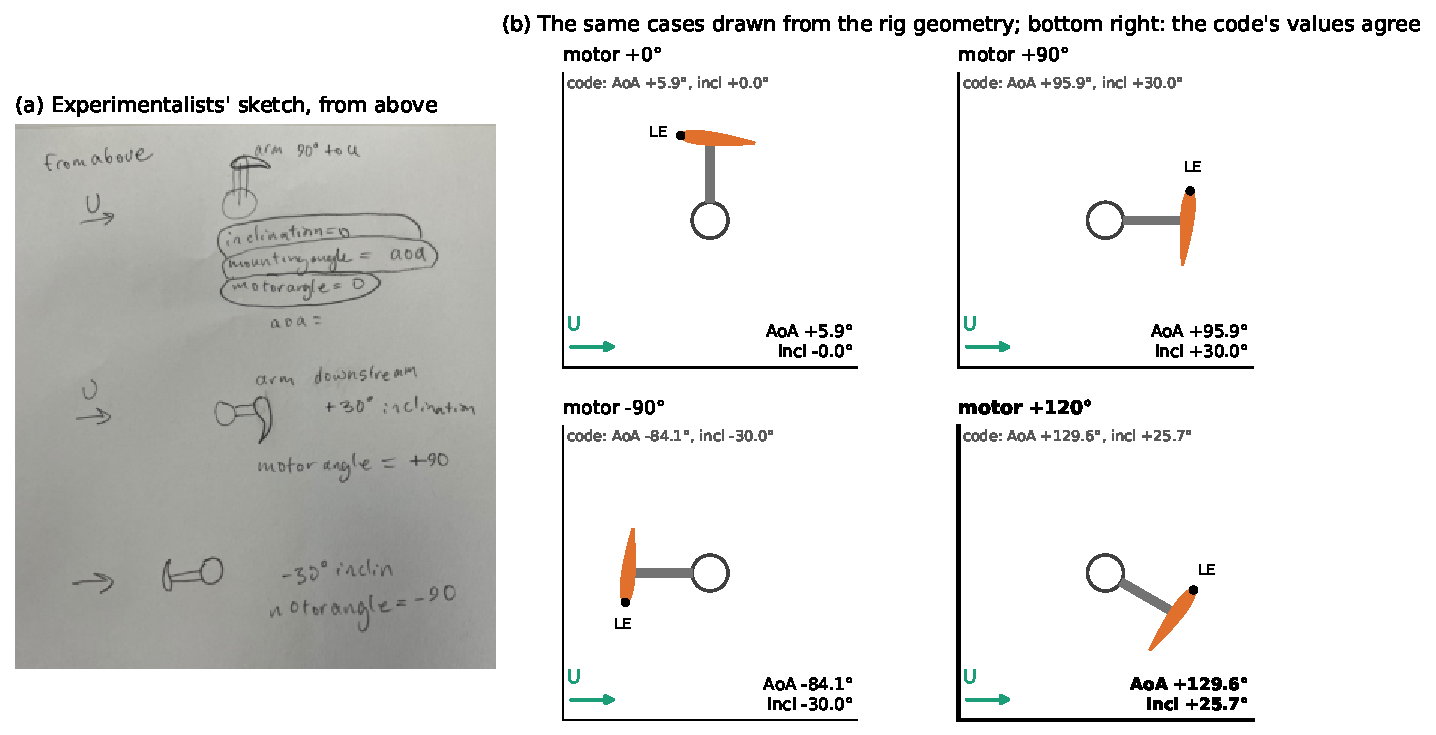
\includegraphics[width=\textwidth]{sketch_vs_geometry.pdf}
  \caption{(a) The experimentalists' sketch (29 September 2026), seen from
  above with the flow ($U$) from left to right: motor 0$^\circ$ (arm across
  the flow, inclination 0), $+90^\circ$ (arm downstream, $+30^\circ$
  inclination) and $-90^\circ$ (arm upstream, $-30^\circ$). (b) The same
  cases and motor 120$^\circ$, drawn from the rig geometry with the blade's
  root section enlarged and the chord at 84.105$^\circ$ to the arm. The
  lower-right numbers come from the vectors; the grey numbers at the top come
  from the fixed code. They agree.}
  \label{fig:sketch}
\end{figure}

\begin{table}[H]
  \centering
  \small
  \begin{tabular}{p{0.2\textwidth}p{0.72\textwidth}}
    \toprule
    Motor angle $\theta$ & 0 puts the arm across the flow. Positive turns
      the arm clockwise seen from above: $+90^\circ$ points it downstream,
      $-90^\circ$ upstream. \\
    Sweep angle $\beta$ & Rotation of the blade's frame from vertical,
      about the horizontal axis perpendicular to the arm. Negative tilts the
      blade tip back toward the shaft. \\
    Mounting angle $\mu$ & Angle between the chord and the arm. $90^\circ$
      means the chord is perpendicular to the arm, which puts it along the
      flow at motor 0. The angle of attack at motor 0 is $90^\circ-\mu$. \\
    Inclination & Angle of the flow out of the blade's cross-section plane.
      Positive when the flow runs along the span from tip to root. \\
    Angle of attack & Angle of the flow, projected into the cross-section
      plane, from the chord (leading edge to trailing edge). Positive toward
      the arm-tip side, so it increases with the motor angle. \\
    \bottomrule
  \end{tabular}
  \caption{Conventions, now stated in the module's docstring.}
  \label{tab:conv}
\end{table}

\begin{figure}[H]
  \centering
  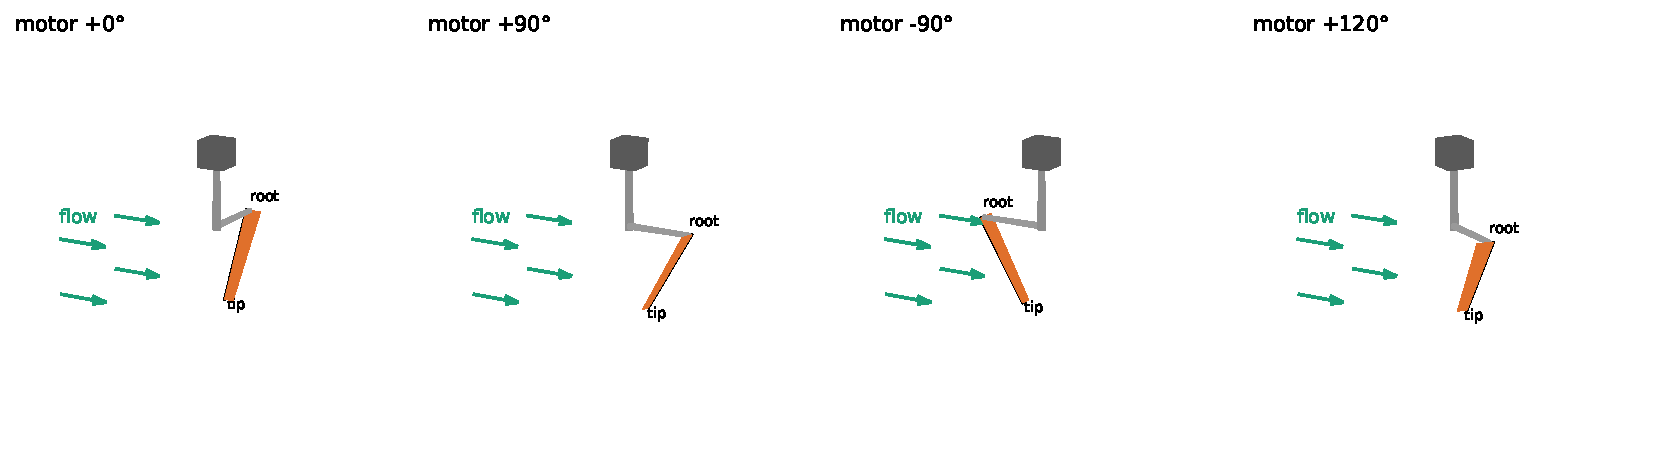
\includegraphics[width=\textwidth]{rig3d.pdf}
  \caption{The rig at the four motor angles of Figure~\ref{fig:sketch}, all
  from the same viewpoint, with the flow from the left. The black line marks
  the leading edge. The chord is drawn three times its size; the arm length
  is illustrative.}
  \label{fig:rig3d}
\end{figure}

%======================================================================
\section{What was wrong}
%======================================================================

The transform works in three frames. The global frame has the flow along
$+x$. The mount frame turns with the motor. The blade (``swept'') frame is
tilted by the sweep angle, with its $z$ axis along the span from tip to
root. The wind components are carried from one frame to the next, then read
off as two angles.

\paragraph{Sweep rotation.} The blade frame is the mount frame rotated by
$\beta$ about the mount $x$ axis. The components of a vector in a rotated
frame transform with the \emph{transpose} of the rotation:
\[
  \mathbf U_s = R_x(\beta)^{\mathsf T}\,\mathbf U_m .
\]
The 1 October version used $R_x(\beta)\,\mathbf U_m$. That is the frame
rotated the other way, a blade leaning with its tip away from the shaft. For
horizontal flow ($w_m = 0$) only the spanwise component changes, and it
changes sign: $w_s = -\sin\beta\,v_m$ instead of $+\sin\beta\,v_m$. So every
inclination had the wrong sign. The angle of attack was unaffected by this
error.

The motor rotation was already right. The mount frame is the global frame
turned clockwise from above, a rotation of $-\theta$ about $z$, and the code's
$R_z(\theta)\,\mathbf U = R_z(-\theta)^{\mathsf T}\mathbf U$ is correct.

\paragraph{Mounting angle.} With the chord at $\mu$ to the arm, the chord lies
$90^\circ-\mu$ from the blade frame's $x$ axis. So
\[
  \alpha = \operatorname{atan2}(v_s, u_s) + (90^\circ - \mu).
\]
The 1 October version added $\mu$ instead. That makes 84.105$^\circ$ the
angle of attack at motor 0, with the chord nearly along the arm. This
contradicts the sketch, which draws the chord along the flow at motor
0$^\circ$, and it shifts every angle of attack by
$2\mu - 90^\circ = 78.21^\circ$.

The collaborator's original code on \code{master} has neither error. It is
written in wind-turbine frames, with the blade's $z$ axis from root to tip
and $\mu$ entered as a pitch, but for horizontal flow it gives the same
angles. The fixed module keeps the rig frames and states their conventions
explicitly. Its function names are unchanged, so every caller picks up the
fix: the summary extractor, the acquisition script and the plotting scripts.

%======================================================================
\section{Checks}
%======================================================================

\begin{figure}[H]
  \centering
  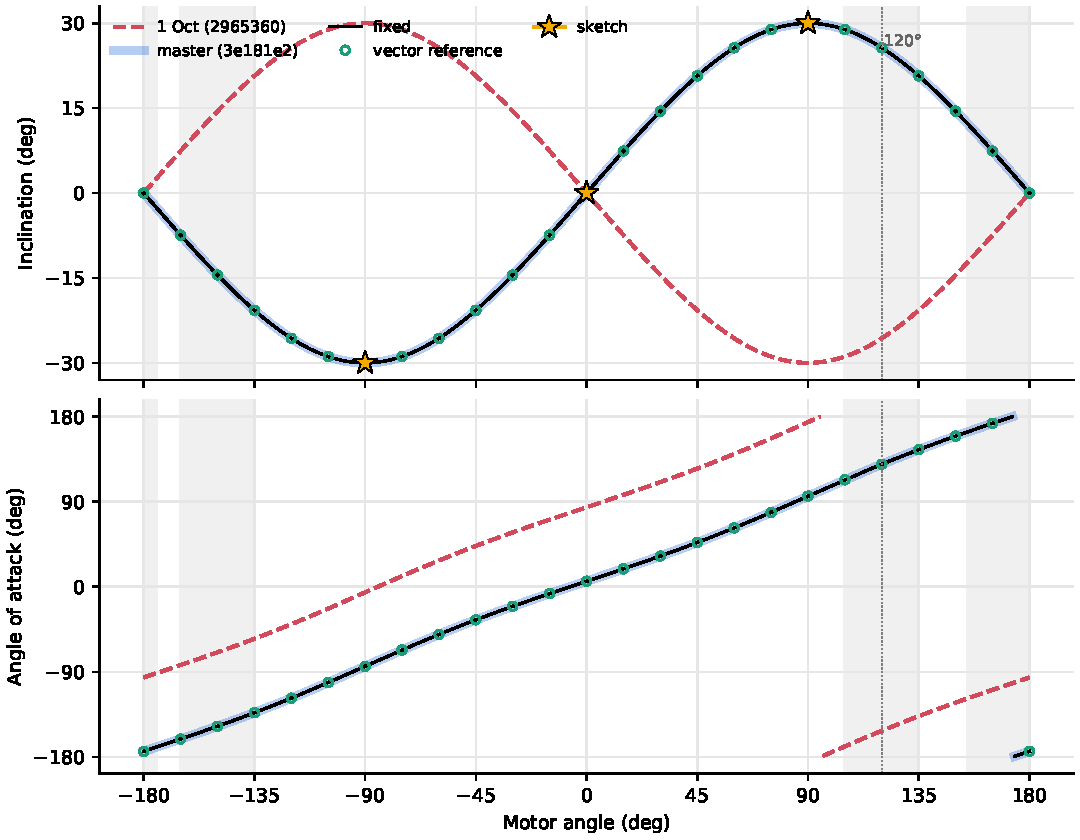
\includegraphics[width=0.85\textwidth]{angles_vs_motor.pdf}
  \caption{Inclination and angle of attack over a full turn of the motor, for
  the production geometry. Black: fixed code. Thick blue: \code{master}
  (hidden under the black line). Dashed red: the 1 October version. Circles:
  the vector construction. Stars: the sketch. Grey bands: vibration regions
  R1--R3 of the PSD-analysis report. Dotted: motor 120$^\circ$.}
  \label{fig:vsmotor}
\end{figure}

\paragraph{1. The sketch.} At motor 0$^\circ$, $+90^\circ$ and $-90^\circ$ the
fixed code gives inclinations 0, $+30^\circ$ and $-30^\circ$, as the sketch
says. The 1 October version gives 0, $-30^\circ$ and $+30^\circ$
(Figure~\ref{fig:vsmotor}, top).

\paragraph{2. An independent construction.} The test file builds the rig from
explicit vectors in the global frame, without the module's rotation
matrices:
\begin{itemize}
  \item the arm direction $\mathbf a$, turning clockwise with the motor;
  \item the tip-to-root axis $\mathbf r = \cos\beta\,\hat{\mathbf z} -
        \sin\beta\,\mathbf a$;
  \item the chord, in the plane normal to $\mathbf r$, at $\mu$ to the arm.
\end{itemize}
The inclination is then $\arcsin(\hat{\mathbf U}\cdot\mathbf r)$, and the
angle of attack is the angle of $\hat{\mathbf U}$ from the chord in that
plane. The comparison grid covers:
\begin{itemize}
  \item every 2.5$^\circ$ of motor angle;
  \item sweeps from $-45^\circ$ to $+45^\circ$;
  \item mounting angles from 60$^\circ$ to 105$^\circ$;
  \item three flow directions, two of them with vertical and lateral
        components. This exercises every term of both rotations, not only the
        horizontal flow of the tunnel.
\end{itemize}
Over these 15\,120 conditions, the fixed code differs from the construction
by at most $6\times10^{-14}$ degrees in inclination and $9\times10^{-14}$
degrees in angle of attack (Figure~\ref{fig:error}). The 1 October version
is off by up to 90$^\circ$ and 120$^\circ$.

\begin{figure}[H]
  \centering
  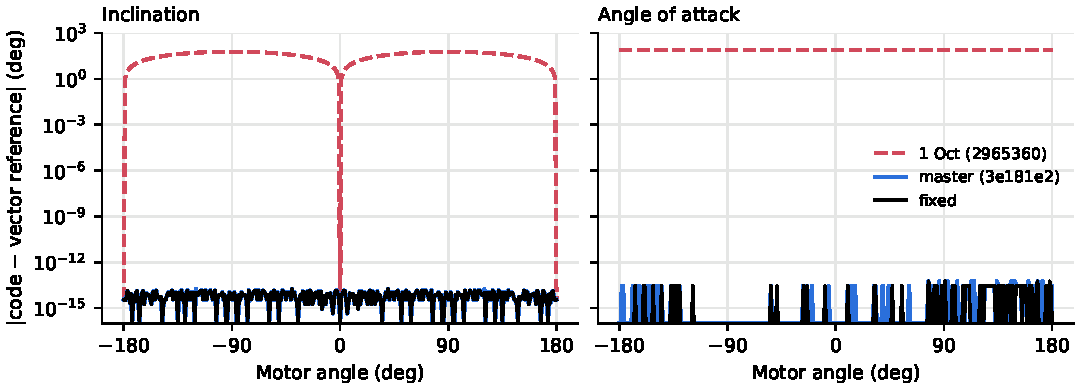
\includegraphics[width=0.85\textwidth]{error.pdf}
  \caption{Difference from the vector construction along the production
  sweep. The fixed code and \code{master} sit at rounding error
  ($10^{-14}$ degrees). The 1 October version is off by twice the
  inclination, and by a constant 78$^\circ$ in angle of attack.}
  \label{fig:error}
\end{figure}

\paragraph{3. The collaborator's code.} A frozen copy of \code{master}'s
transform in the test file agrees with the fixed code to $10^{-9}$ degrees on
the whole grid for horizontal flow. The two differ only when the flow has a
vertical component, because \code{master}'s blade frame stands the blade up
rather than hanging it. The tunnel flow is horizontal, so this never matters
for the data.

\paragraph{4. A hand calculation at motor 120$^\circ$.}
\begin{itemize}
  \item In the mount frame the flow is $(\cos120^\circ, \sin120^\circ, 0) =
        (-0.5, 0.866, 0)$.
  \item For sweep $-30^\circ$, the blade's tip-to-root axis is
        $(0, 0.5, 0.866)$ in mount components. So
        $w_s = 0.433$, and the inclination is
        $\arcsin 0.433 = +25.659^\circ$: tip to root.
  \item The blade frame's $y$ axis is $(0, 0.866, -0.5)$, giving
        $v_s = 0.75$ and $u_s = -0.5$.
  \item The angle of attack is
        $\operatorname{atan2}(0.75, -0.5) + 5.895^\circ = 129.585^\circ$.
\end{itemize}
The code gives exactly these values.

\paragraph{5. Properties any rig must have.} The tests also check that:
\begin{itemize}
  \item a vertical blade sees no inclination;
  \item the inclination never exceeds the sweep, and reaches it when the arm
        lies along the flow;
  \item an arm across the flow gives no inclination;
  \item the angle of attack at motor 0 is $90^\circ - \mu$;
  \item a chord perpendicular to the arm gives $\pm90^\circ$ when the arm
        lies along the flow;
  \item the angle of attack increases with the motor angle;
  \item the mounting angle only shifts the angle of attack;
  \item mirroring the sweep flips the inclination and nothing else.
\end{itemize}

\paragraph{The tests.} \code{scripts/aquire\_data/tests/test\_coordinate\_transforms.py}
holds 21 tests covering points 1--5 and the low-level functions. Together
with the 13 chain tests of Section~\ref{sec:chain}, run them with
\begin{center}
\code{poetry run python -m unittest discover -s scripts/aquire\_data/tests}
\end{center}
All 34 pass on the fixed code. Run against the 1 October code, they fail
in every group: the sketch, the construction, \code{master}, the hand case
and the properties, with 1\,175 failing subtests. Run against
\code{master}, every geometric check passes. The only failures there are
the low-level functions, which \code{master} names differently, and the
non-horizontal flow case.

%======================================================================
\section{The whole chain}
\label{sec:chain}
%======================================================================

The transform is one link. The angles stored with the data pass through
five:
\begin{enumerate}
  \item \code{main.py} sets the run's constants: sweep $-30^\circ$, chord
        offset 5.895$^\circ$, and from it the mounting angle
        $90^\circ - 5.895^\circ$. These are written to
        \code{run\_metadata.json}.
  \item The motor's encoder counts become a motor angle. \code{motor.py}
        converts with $-\text{counts}/694.44$, and so does
        \code{run\_loader.py} when it averages the encoder log over a
        capture. main.py records that average per angle.
  \item \code{coordinate\_transforms} turns the motor angle into the flow
        angles.
  \item During acquisition, main.py writes them to
        \code{coordinate\_frame\_angles.csv}. That was \code{master}'s
        code on the lab PC.
  \item Afterwards, \code{extract\_run\_summary.py} recomputes them into
        \code{angle\_summary.csv} and \code{master\_angles.csv}, which the
        plotting scripts read or recompute in the same way.
\end{enumerate}

\code{tests/test\_angle\_chain.py} checks every link. The data tests run
wherever \code{data/} is present.
\begin{itemize}
  \item \textbf{Constants.} main.py's values are read without importing it,
        since it needs the lab hardware libraries. They give an angle of
        attack of exactly $+5.895^\circ$ and inclination 0 at motor 0, and
        the sketch's $\pm30^\circ$ at $\pm90^\circ$. Every run's metadata
        holds the same values.
  \item \textbf{Encoder sign.} motor.py's two conversions invert each other.
        A synthetic encoder log held at the counts for $+120^\circ$ averages
        to $+120^\circ$ through run\_loader. On the real encoder logs,
        run\_loader's average reproduces the recorded motor angle at every
        one of the 1\,360 captures (Figure~\ref{fig:chain}b). This is the
        link a sign error was fixed in on 2 October (commit
        \code{809a312}).
  \item \textbf{Acquisition against the fixed code.} Every row of every
        \code{coordinate\_frame\_angles.csv} was recomputed from its own
        recorded motor angle with the fixed transform. Inclination and angle
        of attack agree to $3\times10^{-14}$ degrees
        (Figure~\ref{fig:chain}a). This check does not involve the sketch or
        the vector construction: it compares against angles computed during
        the runs, by different code, in different frames.
  \item \textbf{Motor angle reached.} The recorded motor angle is within
        0.7 millidegrees of the requested one at every capture
        (Figure~\ref{fig:chain}c).
  \item \textbf{Summaries.} Every row's motor angle is the one recorded for
        the capture its file holds, and its angles equal the fixed
        transform's. The master table matches the per-run tables.
\end{itemize}

Nine runs measured two angles twice (200$^\circ$ and 210$^\circ$). The
second capture overwrote the first file, so the data at those angles come
from the repeat. Both captures recorded the same motor angle, so the flow
angles are unaffected. The test pairs each summary row with its capture by
the file's start time, not by the requested angle.

\begin{figure}[H]
  \centering
  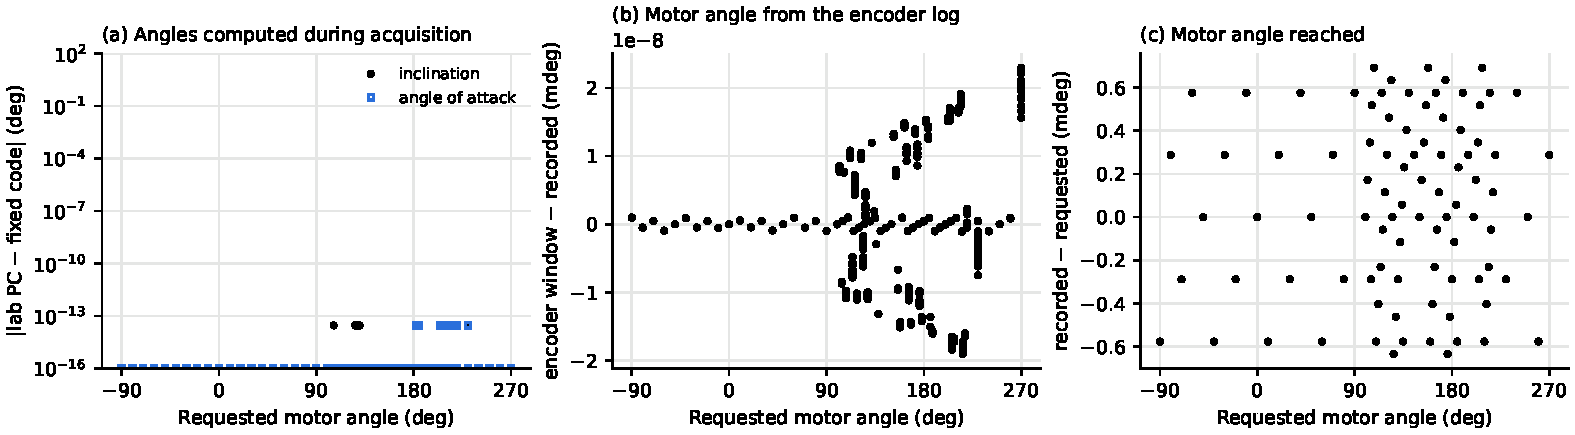
\includegraphics[width=\textwidth]{chain.pdf}
  \caption{The chain on all 1\,360 recorded angles of the 32 production runs.
  (a) Angles computed on the lab PC during acquisition against the fixed code,
  recomputed from the same motor angles; differences are rounding error.
  (b) Motor angle from run\_loader's encoder-window average against the one
  main.py recorded; they agree to $10^{-11}$ degrees. (c) Recorded against
  requested motor angle.}
  \label{fig:chain}
\end{figure}

\paragraph{Also changed.} \code{plot\_regions\_inflow.py} defaulted to sweep
$+30^\circ$ and mounting angle 5$^\circ$, the two substitutions the PSD
report used. Under the fixed conventions those would be wrong, so its
defaults are now the production values. Its region table reproduces the
ranges below. \code{tests/plot\_test\_matrix.py} also uses the production
geometry now.

%======================================================================
\section{Effect on the data}
%======================================================================

\begin{figure}[H]
  \centering
  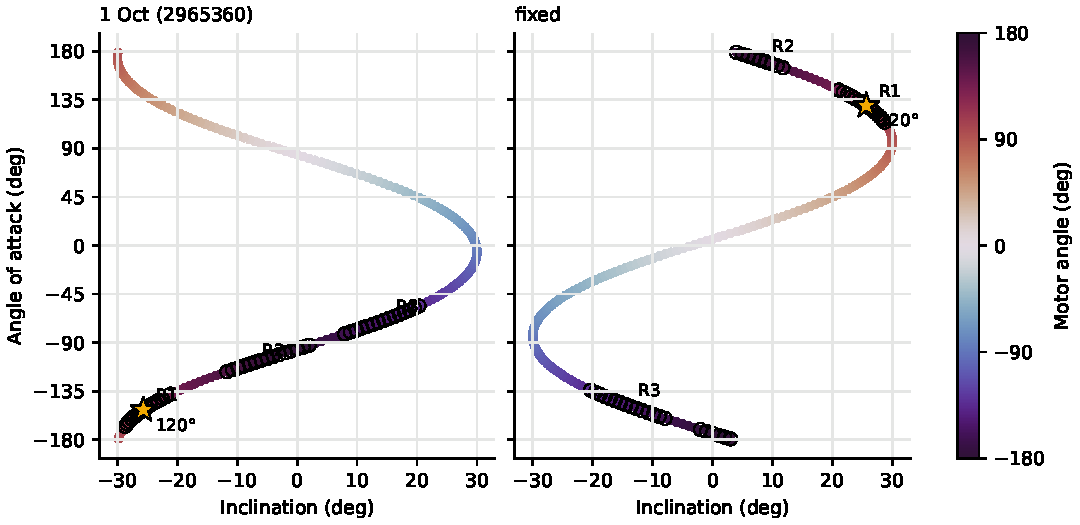
\includegraphics[width=0.85\textwidth]{inflow_map.pdf}
  \caption{The production motor sweep in the inclination--angle-of-attack
  plane, before and after the fix, coloured by motor angle. Circled:
  vibration regions R1--R3. Star: motor 120$^\circ$.}
  \label{fig:map}
\end{figure}

For the production geometry, the fix flips every inclination and lowers every
angle of attack by 78.21$^\circ$ (mod 360$^\circ$). Figure~\ref{fig:map}
shows the effect on the inflow map: the curve is mirrored and shifted, and
the vibration regions move with it. R1 (motor 105--135$^\circ$), which
includes the strongest vibration of the 385\,psi, 6.9\,m/s run at
120$^\circ$, now sits at inclination $+21$ to $+29^\circ$ and angle of
attack $+113$ to $+145^\circ$. The flow comes from the trailing-edge side,
running from tip to root. Before the fix this region read as inclination
$-21$ to $-29^\circ$ and angle of attack $-169$ to $-137^\circ$.

\paragraph{Other reports.} The PSD-analysis report (29 October) gives region
angles that already agree with the fixed code to within 1$^\circ$. It ran
the 1 October code with sweep $+30^\circ$ and mounting angle 5$^\circ$
rather than the recorded $-30^\circ$ and 84.105$^\circ$, and those two
substitutions undo the two errors. Only the parameters it quotes are
misleading. The 120$^\circ$ case report has been updated to the fixed
values.

\paragraph{Summaries.} \code{extract\_run\_summary.py} was rerun on all 32 runs
with the fixed module. Its output was compared with a copy of the old
summaries, using \code{make\_figures.py --before}, over 1\,342 angles in 32
runs:
\begin{itemize}
  \item \code{inclination\_deg}: the new value is minus the old one, to
        $3\times10^{-14}$ degrees.
  \item \code{aoa\_deg}: old minus new is 78.210$^\circ$ (mod 360$^\circ$),
        to $1\times10^{-13}$ degrees.
  \item Every other column of every \code{angle\_summary.csv}, every
        \code{run\_info.json}, all 10\,768 arrays in the \code{spectra.npz}
        files, and the master tables apart from the same two columns are
        bit-for-bit identical.
\end{itemize}
The 385\,psi, fan 800 run at motor 120$^\circ$ now reads inclination
$+25.659^\circ$ and angle of attack $+129.585^\circ$.

\paragraph{Raw run folders.} \code{coordinate\_frame\_angles.csv} in each run
folder was written during acquisition. That code was \code{master}'s, so the
values are right, but they are in \code{master}'s output form: the
unwrapped angle of attack (e.g.\ $-230.4^\circ$ at 120$^\circ$, the same as
$+129.6^\circ$). They were left untouched. Acquisition from now on uses the
fixed module.

%======================================================================
\section{What these checks do not cover}
%======================================================================

The checks establish that the code computes the angles of the rig as
described. They cannot check the description itself. Two inputs rest on
the sketch and on the acquisition code:

\begin{itemize}
  \item \textbf{The mounting angle.} The value comes from
        \code{main.py} on \code{master}: \code{MOUNTING\_ANGLE\_DEG =
        -5.895+90}. On 29 September it was set first to 5.895 (Kyle Devlin,
        ``Setting mounting angle to +5.895'') and then to $90 - 5.895$ (lab
        PC, ``Setting correct mounting angle''), the same day as the sketch.
        So the measured quantity is the 5.895$^\circ$ angle of attack at
        motor 0, the sketch's ``mounting angle = aoa''. The chord is
        5.9$^\circ$ off perpendicular to the arm, which you have confirmed.
        The fixed code reproduces this: $90^\circ - 84.105^\circ =
        5.895^\circ$ at motor 0. The sign of the offset, i.e.\ which way
        the chord is turned from perpendicular, rests on that entry.
  \item \textbf{Which way the leading edge faces.} The sketch draws the
        leading edge upstream at motor 0$^\circ$, and the code assumes this.
        If it faced downstream, every angle of attack would move by
        180$^\circ$.
\end{itemize}

The mean root loads could in principle test both inputs, since the force on
the blade changes direction where the chord lines up with the flow. A first
look puts that crossing at motor $\approx -32^\circ$ and $148^\circ$, about
25$^\circ$ from where the fixed geometry puts it ($-7^\circ$ and
$173^\circ$). That estimate does not separate the blade's force from the
arm's drag, and it assumes an unknown load-cell zero and axis orientation. It
is not evidence either way, but it would be the independent physical check
of the leading-edge direction and of the offset's sign.

\end{document}
